\documentclass[border=10pt]{standalone}
\usepackage{pgfplots}
\pgfplotsset{compat=newest}
\begin{document}
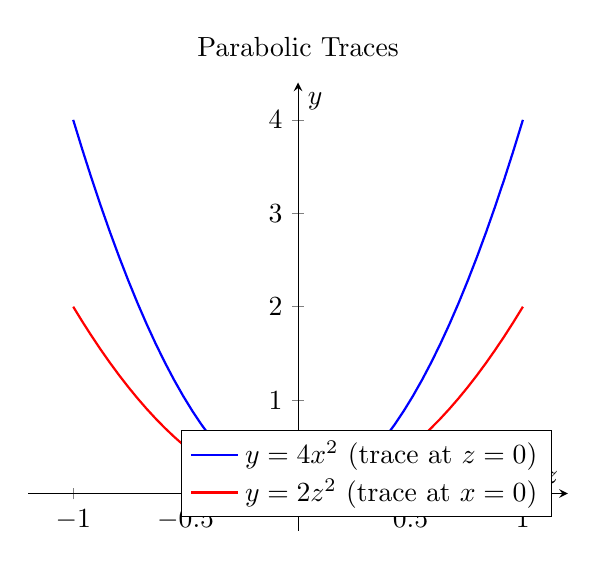
\begin{tikzpicture}
\begin{axis}[
    xlabel={$x$ or $z$},
    ylabel={$y$},
    title={Parabolic Traces},
    domain=-1:1,
    samples=50,
    axis lines=middle,
    enlargelimits=true,
    legend pos=south east
]
\addplot[blue, thick] {4*x^2};
\addlegendentry{$y = 4x^2$ (trace at $z=0$)}

\addplot[red, thick] {2*x^2};
\addlegendentry{$y = 2z^2$ (trace at $x=0$)}

\end{axis}
\end{tikzpicture}
\end{document}